\section{Hybrid 6-bit Floating-Point Computation}
\tableofcontents[currentsection]


\begin{frame}{Case Study: Applying Sensor Analytics to Structural Health Monitoring}
	\begin{columns}[t] % The [T] option aligns the tops of the columns
		
		% Left column for the first image
		\begin{column}<1->{0.5\textwidth}\centering
			\begin{figure}
				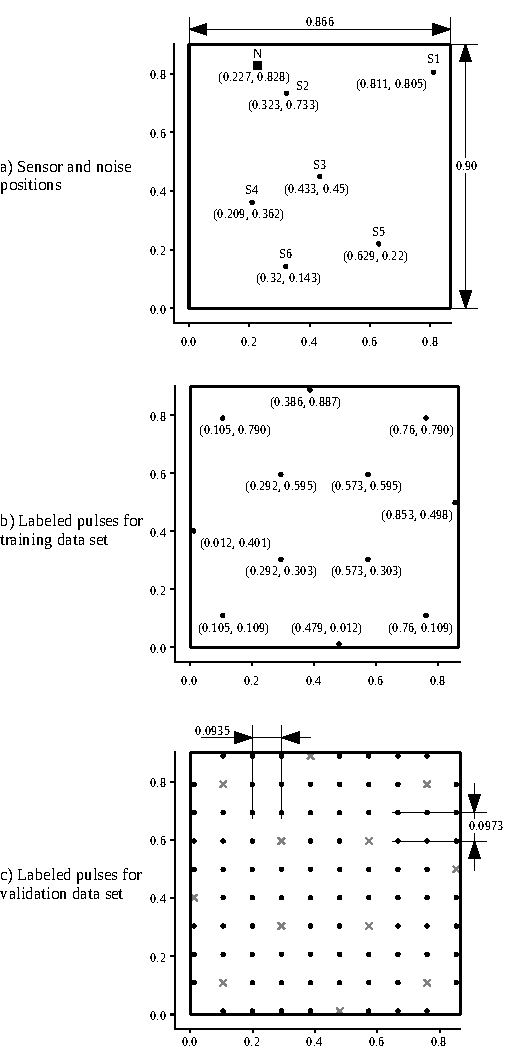
\includegraphics[width=0.5\textwidth]{../chapters/cnn_accelerator/figures/histograms/data_set.pdf} % Adjust the filename
				\caption{ Structural health monitoring, all lengths are in meters (m)}
			\end{figure}
		\end{column}
		
		% Right column for the second image
		\begin{column}<2->{0.5\textwidth}
			\begin{figure}
				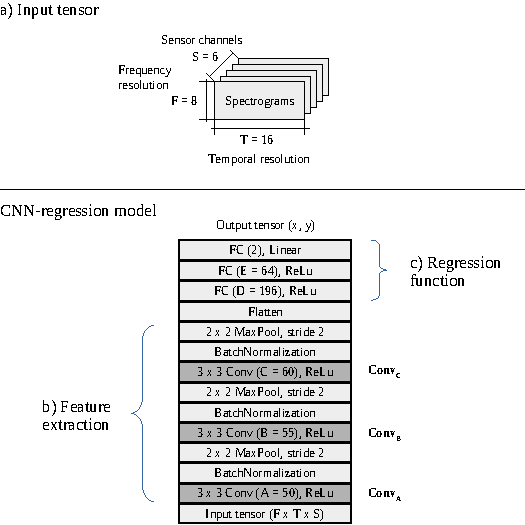
\includegraphics[width=0.75\textwidth]{../chapters/cnn_accelerator/figures/models.pdf} % Adjust the filename
				\caption{ CNN-regression model for sensor analytics}
			\end{figure}
		\end{column}
		
	\end{columns}
\end{frame}


\begin{frame}{Evaluating Floating-Point Configurations: Speed, Power, and Hardware Utilization}
	% Using columns to arrange images vertically in two columns
	\begin{columns}[T] % Align columns at the top
		\begin{column}{0.5\textwidth}
			\centering
			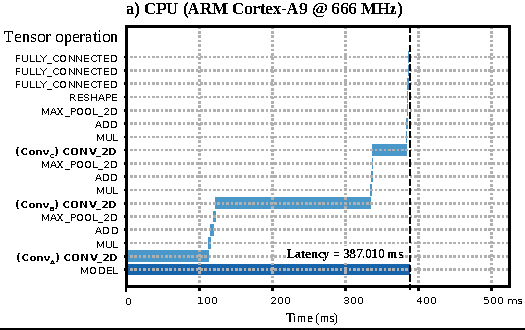
\includegraphics[width=0.5\linewidth]{slides/figures/runtime_a.pdf} % Left top image
			\pause % Wait to reveal the next image
			
			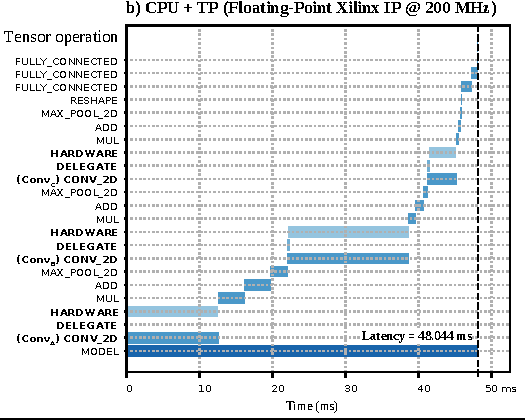
\includegraphics[width=0.5\linewidth]{slides/figures/runtime_b.pdf} % Left middle image
			\pause % Wait to reveal the next image
			
			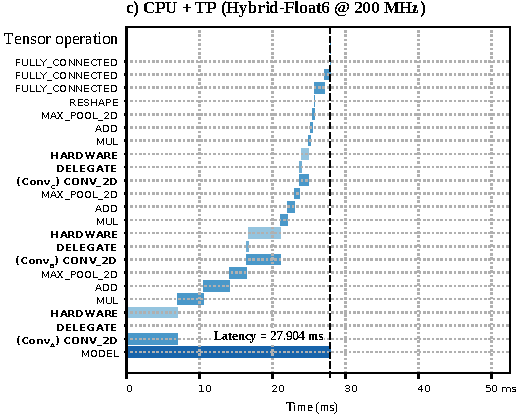
\includegraphics[width=0.5\linewidth]{slides/figures/runtime_c.pdf} % Left bottom image
			\pause % Wait to reveal the next image
		\end{column}
		
		\begin{column}{0.5\textwidth}
			\centering
			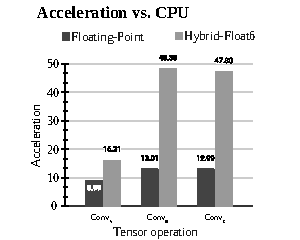
\includegraphics[width=0.5\linewidth]{slides/figures/acceleration_vs_cpu.pdf} % Right top image
			\pause % Wait to reveal the next image
			
			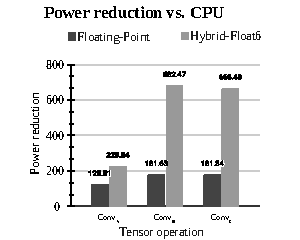
\includegraphics[width=0.5\linewidth]{slides/figures/power_reduction_vs_cpu.pdf} % Right middle image
			\pause % Wait to reveal the next image
			
			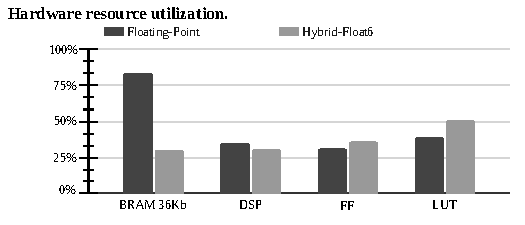
\includegraphics[width=0.8\linewidth]{slides/figures/resource_utilization.pdf} % Right bottom image
		\end{column}
	\end{columns}
\end{frame}


\begin{frame}{Quantization Impact: Error Histograms in Position Prediction}
	% Using columns to arrange images
	\begin{columns}[T] % Align columns at the top
		\begin{column}{0.5\textwidth}
			\centering
			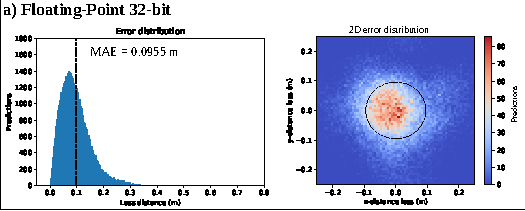
\includegraphics[width=0.95\linewidth]{slides/figures/model_evaluation_a.pdf} % Left top image
			\pause % Wait to reveal the next image
			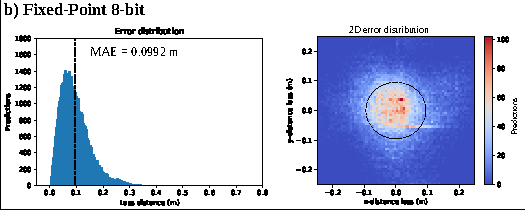
\includegraphics[width=0.95\linewidth]{slides/figures/model_evaluation_b.pdf} % Left middle image
			\pause % Wait to reveal the next image
			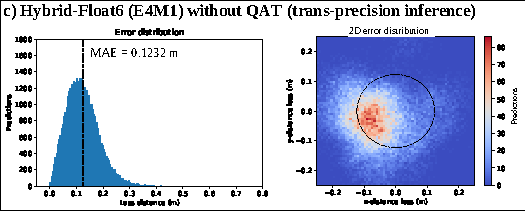
\includegraphics[width=0.95\linewidth]{slides/figures/model_evaluation_c.pdf} % Left bottom image
			\pause % Wait to reveal the next image
		\end{column}
		
		\begin{column}{0.5\textwidth}
			\centering
			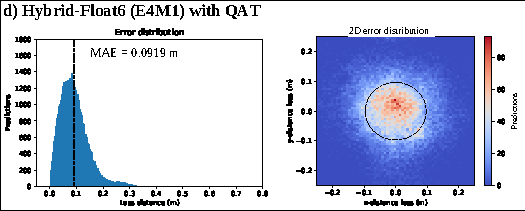
\includegraphics[width=0.95\linewidth]{slides/figures/model_evaluation_d.pdf} % Right top image
			\pause % Wait to reveal the next image
			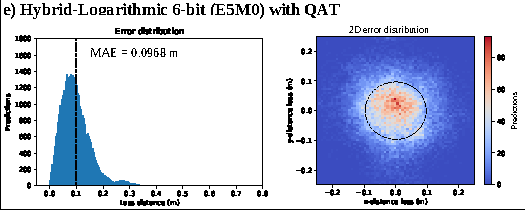
\includegraphics[width=0.95\linewidth]{slides/figures/model_evaluation_e.pdf} % Right middle image
			\pause % Wait to reveal the next image
			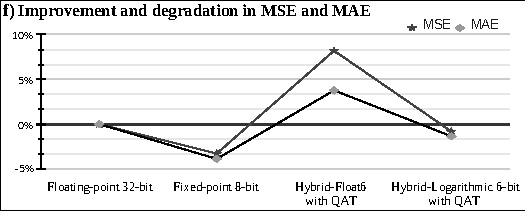
\includegraphics[width=0.95\linewidth]{slides/figures/model_evaluation_f.pdf} % Right bottom image
		\end{column}
	\end{columns}
\end{frame}
